%--------------------------------------------------------------------
%--------------------------------------------------------------------
% Formato para los talleres del curso de Métodos Computacionales
% Universidad de los Andes
%--------------------------------------------------------------------
%--------------------------------------------------------------------

\documentclass[11pt,letterpaper]{exam}
\usepackage[utf8]{inputenc}
\usepackage[spanish]{babel}
\usepackage{graphicx}
\usepackage{tabularx}
\usepackage[absolute]{textpos} % Para poner una imagen en posiciones arbitrarias
\usepackage{multirow}
\usepackage{float}
\usepackage{hyperref}
%\decimalpoint

\begin{document}
\begin{center}
{\Large Métodos Computacionales} \\
\textsc{Tarea 2}\\
Maria Camila Garcia 201515657\\
11-02-2019\\
\end{center}

En la siguiente figura se presenta la grafica de los datos signal.dat y signalSuma.dat.

\noindent
\section{Ejercicio 1: Fourier}
\begin{center}
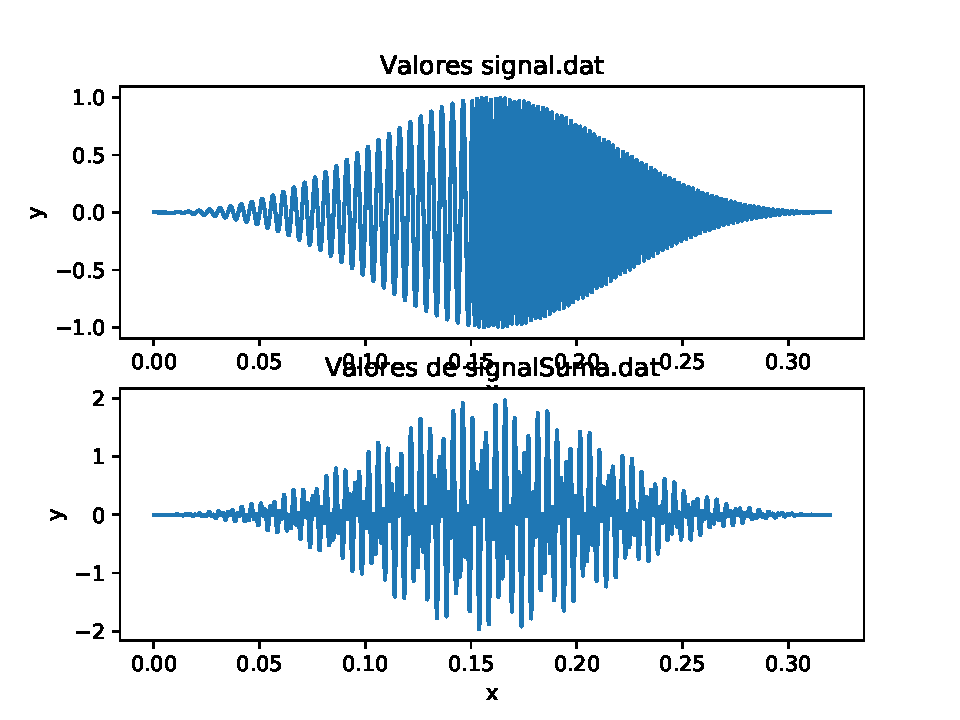
\includegraphics[width=10cm]{GarciaCamila_SubplotsGraficas.pdf}
\end{center}

A continuacion se tienen la grafica de de las transformadas de fourier para ambas señales. 

\begin{center}
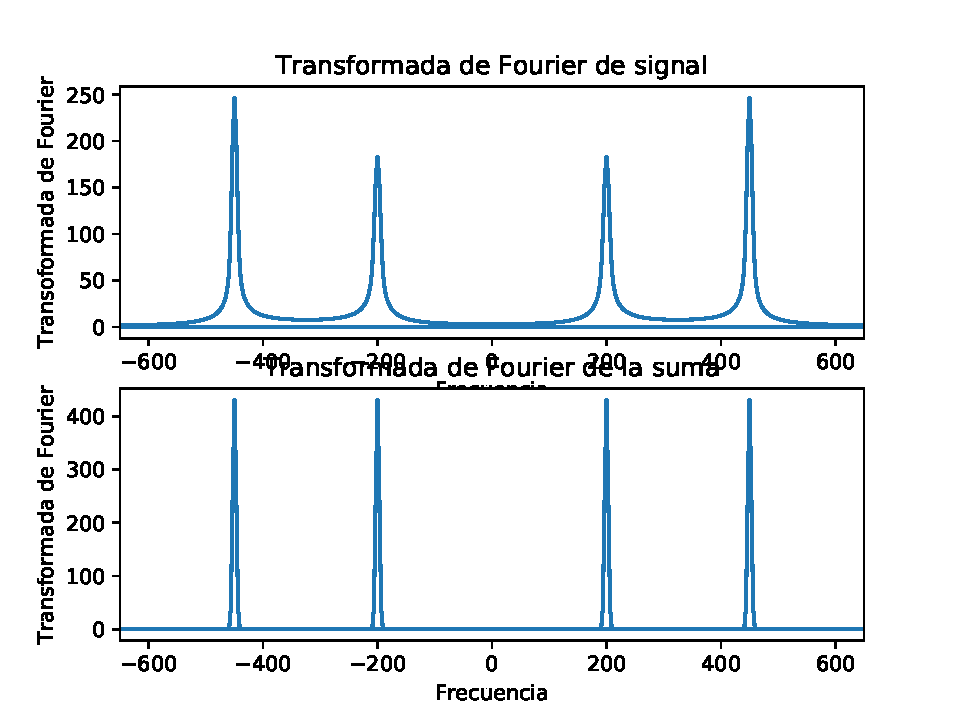
\includegraphics[width=10cm]{GarciaCamila_Transformadas.pdf}
\end{center}

Posteriormente, se muestra el espectrograma de los datos signal.dat y signalSuma.dat.

\begin{center}
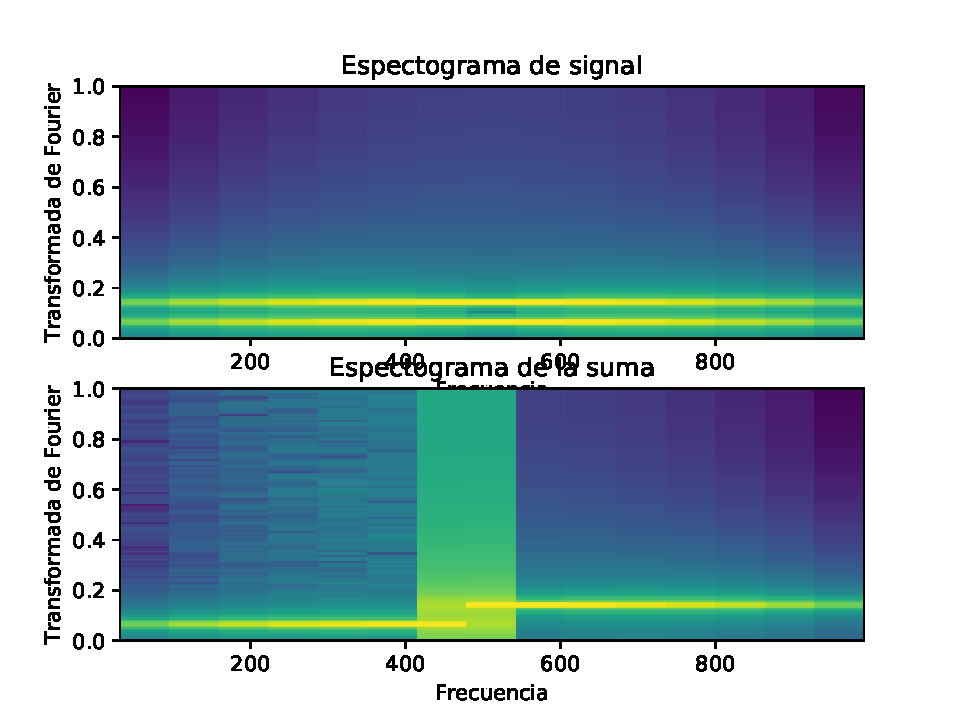
\includegraphics[width=10cm]{GarciaCamila_Espectrogramas.pdf}
\end{center}

Respecto al espectrograma, pordemos decir que para el caso del temblor, este busca medir el movimiento de la estructura ante la vibracion del suelo que soporta. En general, representa la energia del contenido de la señal, por lo que hace un trabajo muy similar al de la transformada de Fourier. 

En la grafica de la señal en funcion del tiempo de temblor.txt se tiene:

\noindent
\section{Ejercicio 2: Ecuaciones diferenciales ordinarias: un edificio en un sismo}

Grafica de la amplitud maxima en funcion de w. 
\begin{center}
\includegraphics[width=10cm]{GarciaCamila_Amplitudui(t)maxVsW.pdf}
\end{center}

\begin{center}
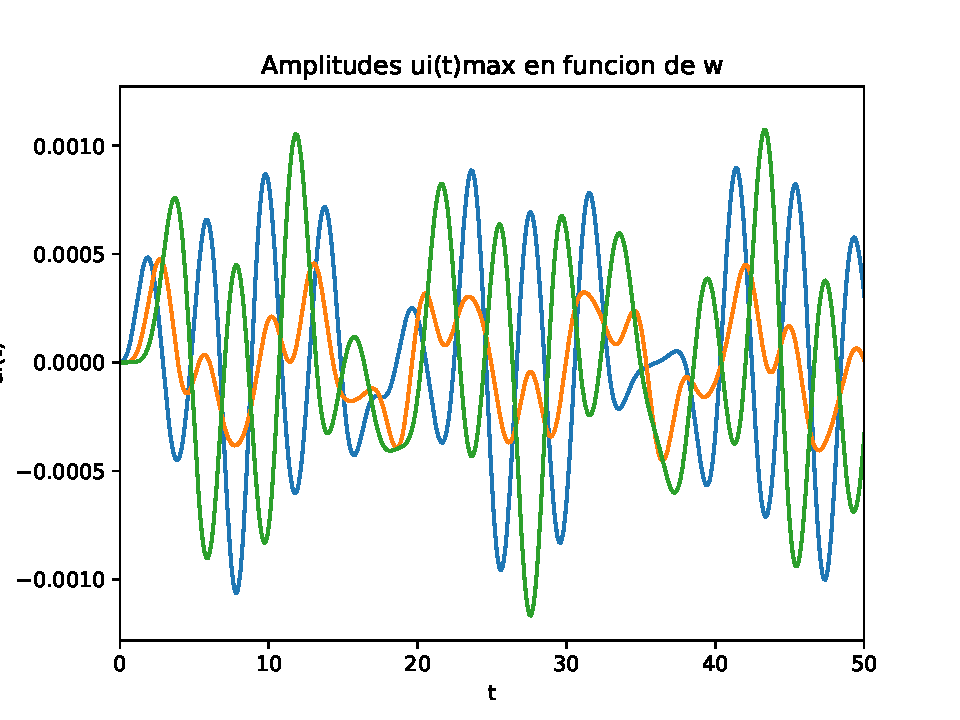
\includegraphics[width=10cm]{PrimeraGraficaUi(t).pdf}
\end{center}

\begin{center}
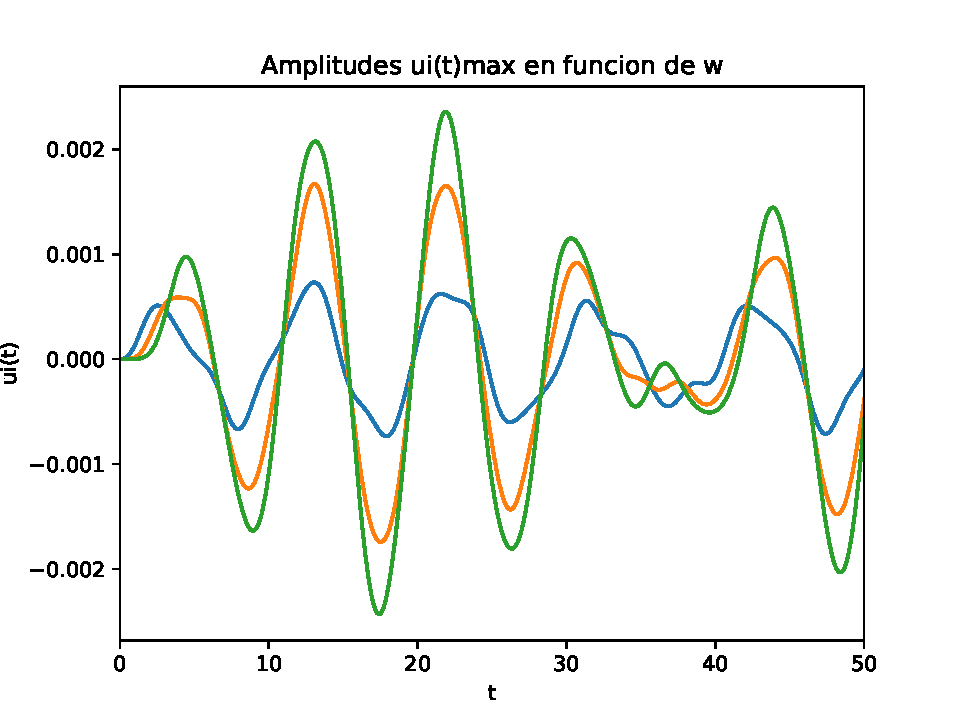
\includegraphics[width=10cm]{SegundaGraficaUi(t).pdf}
\end{center}

\begin{center}
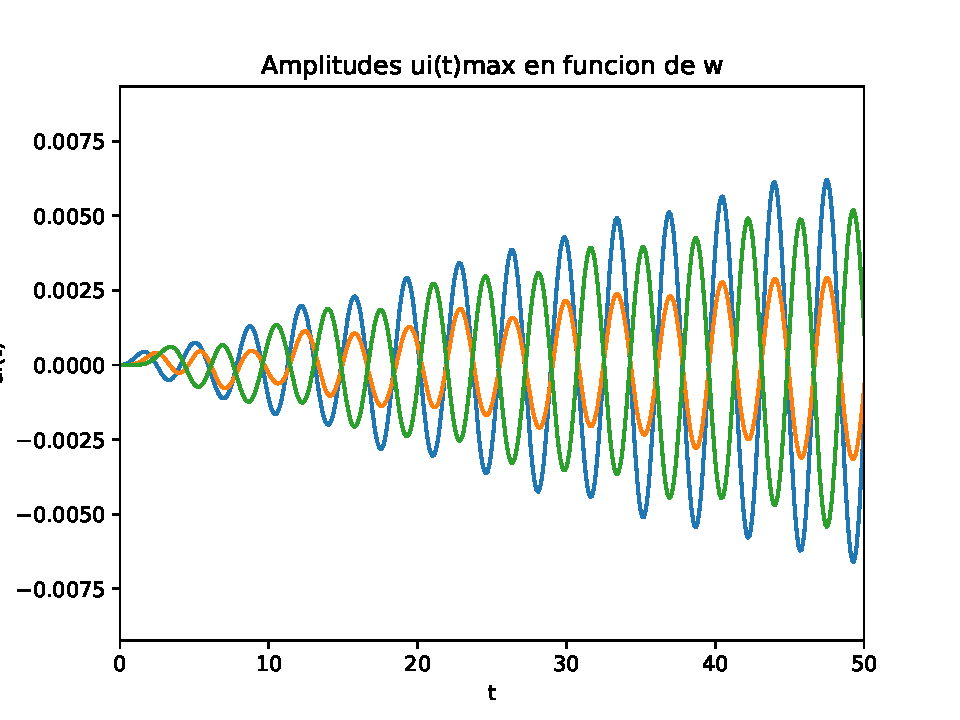
\includegraphics[width=10cm]{TerceraGraficaUi(t).pdf}
\end{center}

\begin{center}
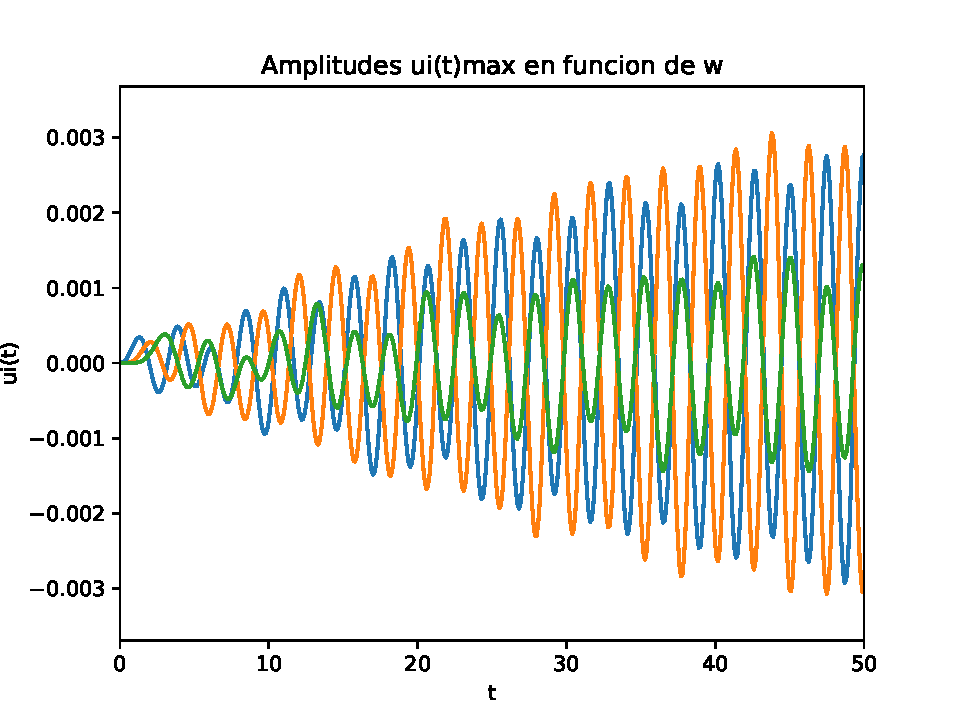
\includegraphics[width=10cm]{CuartaGraficaUi(t).pdf}
\end{center}

\end{document}
